\documentclass[landscape,twocolumn]{article}
\usepackage{german}
\usepackage[latin1]{inputenc}
\usepackage{dcolumn}
\usepackage{longtable}
\usepackage{amsmath}
\usepackage{amssymb}
\usepackage{wrapfig}
\usepackage{epsfig}
\usepackage{fancyheadings}
\usepackage{multirow}

\textheight=16.2cm \textwidth=25 cm \evensidemargin=\oddsidemargin
\setlength{\headsep}{25pt}


\font \tams  = cmmib10   scaled \magstep1 \font \tamss =cmmib10
\font \tenbfne = cmb10   scaled \magstep1 \font \sevenbfne = cmb10
\def\vek#1{\ifmmode{\textfont1=\tams\scriptfont1=\tamss
              \textfont0=\tenbfne\scriptfont0=\sevenbfne
              \mathchoice{\hbox{$\displaystyle#1$}}{\hbox{$\textstyle#1$}}
              {\hbox{$\scriptstyle#1$}}{\hbox{$\scriptscriptstyle#1$}}}
             \else \vrule width 4pt\ #1\ \fi}




 \setlength{\parindent}{0pt}
 \setlength{\voffset}{-0.8in}
 \setlength{\hoffset}{-0.088in}
 \setlength{\columnsep}{1cm}


\begin{document}
\pagestyle{fancyplain}
 \lhead[]{\large  Physikalisches
Anf\"{a}ngerpraktikum der Universit\"{a}t Heidelberg - Praktikum II} \rhead{\large Versuch 252 Aktivierung von Indium und Silber}

\cfoot{\large\vspace{0.1in}$\qquad$\rm\thepage}
\lfoot{\copyright~Dr. J.Wagner - Physikalisches Anf\"{a}ngerpraktikum
-~V.~1.5~Stand~03/2012} \setlength{\footrulewidth}{0.4pt}
\renewcommand{\thesection}{\Roman{section}}


\begin{center}
\LARGE\bf{Versuch 252\\ Aktivierung von Indium und von Silber mit thermischen Neutronen}
\end{center}

\begin{figure}[h]
\begin{minipage}[c]{12cm}
\centering\epsfig{file=252_aufbau.eps,width=\textwidth}
\caption{\fontsize{10}{12}\it Oben: Versuchsaufbau. Unten: Neutronenquelle.}
\end{minipage}
\end{figure}


\section{Messaufbau}
\begin{itemize}
 \item  Geiger-M\"{u}ller Z\"{a}hlrohr mit Betriebsger\"{a}t
 \item  Externer Impulsz\"{a}hler
 \item PC mit Drucker
 \item Neutronenquelle
 \item Pr\"{a}paratehalterung
 \item Indium- und Silberbleche
\end{itemize}



\section{Vorbereitung}
Bereiten Sie sich  auf die Beantwortung von Fragen zu folgenden
Themen vor: Radioaktiver Zerfall, Zerfallsarten, Nuklide,
Geiger-M\"{u}ller-Z\"{a}hlrohr.\\
\\Verst\"{a}ndnisfragen:
\begin{enumerate}
\item Was ist ein Neutron?
\item Was passiert, wenn ein Atomkern ein langsames Neutron einf\"{a}ngt?
\item Wie ist der Zusammenhang zwischen Aktivierung und Zerfall?
\item Was ist die Halbwertszeit, wie kann man sie messen?
\item Wie sieht das Spektrum eines $\beta$-Strahlers aus? Warum handelt es sich um ein
kontinuierliches Spektrum?
\end{enumerate}

\section{Aufgaben}
\begin{enumerate}
\item Bestimmung der Halbwertszeit von $^{116}$In.
\item Bestimmung der Halbwertszeiten von $^{108}$Ag und $^{110}$Ag
\end{enumerate}

\section{Grundlagen}


Zur Herstellung einer radioaktiven Quelle werden stabile Isotope durch Kernreaktionen aktiviert. Besonders geeignet
hierf\"{u}r sind Neutronen, da diese nicht der Coulomb-Wechselwirkung ausgesetzt sind und daher vom Kern leicht eingefangen werden k\"{o}nnen.
In diesem Versuch werden die Isotope $^{115}$In bzw. $^{107}$Ag / $^{109}$Ag mit Hilfe thermischer Neutronen aktiviert.

Die Neutronenquelle besteht aus
einem Pr\"{a}parat, das Berylliumsp\"{a}ne und einen  $\alpha$-Strahler
($^{241}$Am) enth\"{a}lt. Durch die Kernreaktion
\begin{equation}\notag
  ^{9}\text{Be} + \alpha \rightarrow ^{12}\text{C} + \text{n}
\end{equation}
entstehen Neutronen mit einer Energie von 1 - 10~MeV. Diese
schnellen Neutronen werden in dem die Neutronenquelle umgebenden
Paraffinblock durch elastische St\"{o}{\ss}e mit den Wasserstoffkernen
abgebremst, bis sie nahezu thermische Energie erreicht haben.
St\"{o}{\ss}e gegen die Kohlenstoffkerne bremsen die Neutronen nur wenig
ab. Bei einem elastischen Sto{\ss} gegen eine gleich schwere Masse
(n\"{a}mlich gegen ein Proton) verliert dagegen das Neutron im Mittel
die H\"{a}lfte der Energie. Viele Atomkerne haben einen gro{\ss}en
Wirkungsquerschnitt f\"{u}r den Einfang langsamer Neutronen. Dabei
entsteht ein Isotop des bestrahlten Elements mit einer um eins
erh\"{o}hten Massenzahl. Wenn dieser Kern radioaktiv ist, stellt die
Aktivierung durch langsame Neutronen die bequemste M\"{o}glichkeit zur
Erzeugung dieses radioaktiven Isotops dar. Bei Bestrahlung von Indium
wird aus dem stabilen Isotop $^{115}$In der $\beta$-Strahler $^{116}$In gebildet.
Allerdings werden dabei zwei sogenannte Isomere erzeugt.
Dabei handelt es sich um Nuklide, die jeweils die gleiche Anzahl von Neutronen und Protonen besitzen, sich aber in einem unterschiedlichen
Energiezustand befinden. Zum einen wird $^{116}$In gebildet welches sich im Grundzustand befindet, zum anderen
der metastabile Zustand $^{116m}$In. Beide Nuklide sind $\beta^-$-Strahler die mit unterschiedlichen Halbwertszeiten in das
stabile Isotop $^{116}$Sn zerfallen. Die Halbwertszeiten finden Sie in der Nuklidkarte im Anhang.

\begin{figure}[h]
\begin{minipage}[c]{12cm}
\centering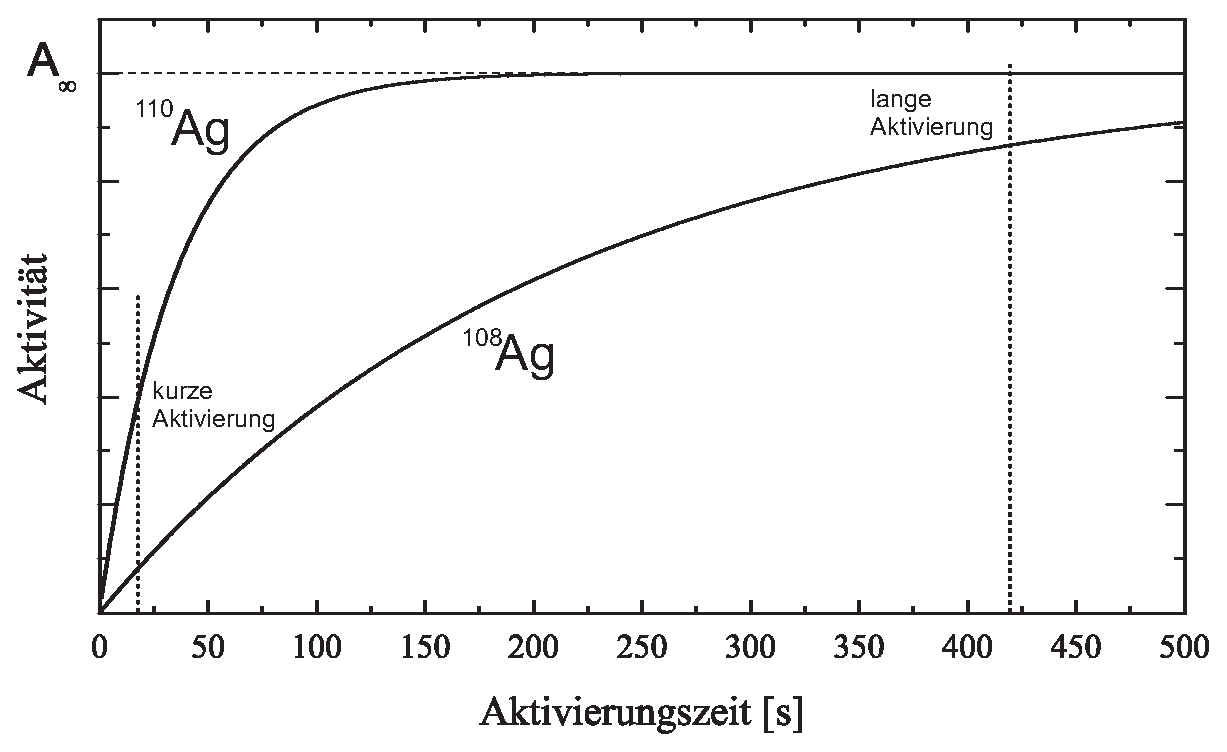
\epsfig{file=252_aktivierung_silber.eps,width=\textwidth}
\caption{\label{252_ag}\fontsize{10}{12}\it Aktivit\"{a}t von $^{108}$Ag und $^{110}$Ag bei unterschiedlichen Aktivierungszeiten. Es wurde angenommen, dass der
Wirkungsquerschnitt bei beiden Isotopen identisch ist.}
\end{minipage}
\end{figure}

Bei der Aktivierung wird pro Sekunde eine bestimmte Zahl von
radioaktiven Kernen erzeugt. Die Zahl der pro Sekunde zerfallenden
Kerne ist aber der Anzahl der jeweils vorhandenen radioaktiven
Kerne proportional (Zerfallsgesetz). Daher nimmt die Aktivit\"{a}t $A$
(d.h. die Zahl der Zerf\"{a}lle pro Sekunde) als Funktion der
Bestrahlungsdauer $t$ nach dem Gesetz

\begin{equation}
A(t) = A_\infty (1 - \exp\{ - \lambda t\} )
\end{equation}

zu, bis ein Gleichgewicht eintritt, bei dem pro Sekunde gleichviel
Kerne des radioaktiven Isotops neu gebildet werden wie pro Sekunde
zerfallen. Nach Ende der Aktivierung tritt dann nur noch der
Zerfall nach dem radioaktiven Zerfallsgesetz
\begin{equation}
A(t) = A_0\, \exp{( - \lambda t)}
\end{equation}
auf. F\"{u}r die Halbwertszeit gilt
\begin{equation}
T_{1/2} =\frac{\ln 2}{\lambda}.
\end{equation}


Da nat\"{u}rliches Silber aus 51\% $^{107}$Ag und
49\% $^{109}$Ag besteht, werden bei der Aktivierung  zwei unterschiedliche Isotope erzeugt. Es entstehen die radioaktiven
Silberisotope $^{108}$Ag und $^{110}$Ag. Sie zerfallen durch $\beta$-Zerfall in $^{108}$Cd und $^{110}$Cd. Da die Halbwertszeiten dieser Silber-Isotope sich
um etwa einen Faktor~6 unterscheiden, kann durch unterschiedlich lange Aktivierungszeiten das Isotopenverh\"{a}ltnis variiert werden. Wird nur kurz aktiviert (20~s),
entsteht vor allem $^{110}$Ag. Mit zunehmender Aktivierungszeit wird vermehrt $^{108}$Ag erzeugt w\"{a}hrend $^{110}$Ag in S\"{a}ttigung geht (Abbildung \ref{252_ag}).

\section{Durchf\"{u}hrung des Versuchs}

\begin{enumerate}
\item \it Halbwertszeit von Silber\rm \\
\bf Achtung: Die bereits aktivierten Indiumpr\"{a}parate d\"{u}rfen w\"{a}hrend dieser Messung nicht aus der Neutronenquelle entfernt werden! F\"{u}r die Aktivierung der Silberpr\"{a}parate sind gen\"{u}gend freie Steckpl\"{a}tze vorhanden.\rm

Stellen Sie am Betriebsger\"{a}t die Z\"{a}hlrohrspannung zwischen 500~V bis 550~V ein.
Bestimmen Sie zun\"{a}chst den Untergrund. Entfernen Sie alle Quellen aus dem Raum. Stellen Sie im
Messprogramm \verb"zerfall.exe" die Torzeit des Z\"{a}hlers auf 10~Sekunden und messen Sie \"{u}ber einen Zeitraum von 8 Minuten den Untergrund.
Speichern Sie die Messdaten unter einem geeigneten Namen, z.B. \verb"UntergrundAgxx.dat" wobei Sie f\"{u}r \verb"xx" Ihre Initialen w\"{a}hlen.

F\"{u}r die Silbermessung wird wieder eine Torzeit von 10~Sekunden eingestellt. Lassen Sie sich vom Assistenten zeigen, wie man die Tr\"{a}ger mit den Silberblechen
(blaues Tr\"{a}germaterial) in die Neutronenquelle einlegt. Das Silberblech wird mindestens 7~Minuten lang aktiviert
und dann \bf so schnell wie m\"{o}glich\rm~vor das Z\"{a}hlrohr gebracht. Stecken Sie das Pr\"{a}parat mit der Silberseite
zum Z\"{a}hlrohr hin in die vorgesehene Aussparung und fixieren Sie es mit dem Aluminiumblech. Starten Sie sofort das
Messprogramm durch einen Mausklick auf den Pfeil im linken oberen Bereich des Programmfensters. Die gesamte Messzeit sollte 400~Sekunden betragen.
\bf Wiederholen Sie die Messung mit der gleichen Probe dreimal. Insgesamt sollen die Z\"{a}hlraten f\"{u}r vier Aktivierungszyklen gemessen werden.\rm~
Speichern Sie jedes Mal die Messdaten und drucken Sie das Protokoll aus.

\item \it Halbwertszeit von Indium\rm \\

Stellen Sie im Messprogramm das Messintervall auf 120~s und stecken Sie das aktivierte Indium- Pr\"{a}parat (rotes Tr\"{a}germaterial) in die Halterung.
Die Messung sollte \"{u}ber einen Zeitraum von 50~Minuten gehen. Speichern Sie am Ende der Messung die Daten und drucken Sie das Protokoll aus.
W\"{a}hrend die Indiummessung l\"{a}uft, k\"{o}nnen Sie bereits mit der Auswertung der Silbermessung beginnen.



\end{enumerate}

\section{Auswertung}
Achtung: Da es im Laborbuch nicht m\"{o}glich ist nachzuvollziehen, welche Rechnungen Sie mit Origin durchgef\"{u}hrt haben, muss bei allen Spaltenberechnungen die entsprechende Rechenvorschrift (Formel) im Laborbuch kommentiert werden.
\begin{enumerate}
\item Zerfall der Silberisotope:\\
\\
Untergrundbestimmung:\\
\\
\"{O}ffnen Sie ein neues Projekt und Importieren Sie die Daten der Untergrundsmessung:
\verb"Datei" $\rightarrow$ \verb"Import" $\rightarrow$ \verb"Einzelnes ASCII".
Wir brauchen im Weiteren nur den Mittelwert und Fehler der Untergrundrate in einem 10~s Intervall. Dieses kann mit Origin leicht mit der Spaltenstatistik bestimmt werden. Hierzu die Spalte mit den Z\"{a}hlraten durch Linksklick auf den Spaltenkopf markieren und mit Rechtsklick \verb"Statistik" $\rightarrow$ \verb"Spaltenstatistik" ausw\"{a}hlen. W\"{a}hlen Sie im folgenden Fenster die gew\"{u}nschten Gr\"{o}{\ss}en aus. Notieren Sie den Mittelwert und dessen Fehler im Laborbuch.

Bestimmung der Zerfallskonstanten:\\
\\
\"{O}ffnen Sie eine neue Arbeitsmappe und lesen Sie die Daten der vier Zerfallsmessungen \"{u}ber 5~Minuten in dasselbe Datenblatt ein.
Hierzu \verb"Datei" $\rightarrow$ \verb"Import" $\rightarrow$ \verb"Mehrere ASCII" ausw\"{a}hlen. W\"{a}hlen Sie die vier Messdateien aus, klicken Sie auf \verb"Hinzufuegen"  und anschlie{\ss}end auf \verb"OK". Sie haben nun vier einzelne Arbeitsmappen, wobei die erste Spalte die Nummer der Messung angibt und die zweite die Zahl der gemessenen Zerf\"{a}lle. Da die Messeinstellung im Experiment f\"{u}r alle vier Messungen gleich war (gleiche L\"{a}nge des Zerfallsintervalls und gleiche Zahl der Messungen), brauchen Sie von drei Messungen jeweils nur die zweite Spalte. Erzeugen Sie in einer Arbeitsmappe drei zus\"{a}tzliche Spalten und f\"{u}gen Sie in diese die Messdaten (zweite Spalte) der drei anderen Arbeitsmappen ein. Dazu einfach die jeweilige Spalte durch Linksklick auf den Spaltenkopf markieren und mit Rechtsklick die Option \verb"Kopieren" ausw\"{a}hlen. Genauso verfahren Sie zum Einf\"{u}gen der Daten in die andere Arbeitsmappe. Die drei Arbeitsmappen k\"{o}nnen Sie anschlie{\ss}end l\"{o}schen.

In der ersten Spalte steht die jeweilige Messnummer. Wir ben\"{o}tigen aber die mittlere Zerfallszeit jedes Intervalls. Markieren Sie diese Spalte und w\"{a}hlen Sie durch Rechtsklick die Option  \verb"Spaltenwerte errechnen...". F\"{u}hren Sie f\"{u}r ein Intervall von 10 Sekunden folgende Berechnung durch:  \verb"col(A)*10 - 5." Beschriften Sie anschlie{\ss}end alle Spalten mit sinnvollen Namen und Einheiten.

Erstellen Sie zwei neue Spalten mit der Summe der Zerfallsereignisse aller vier Messungen und mit dem Fehler dieser Zerfallszahlen (sqrt(NZerf\"{a}lle)). Die Tabelle sollte in etwa so wie in Abbildung~\ref{252_soft1} dargestellt aussehen.

\begin{figure}[h]
\begin{minipage}[c]{12cm}
\centering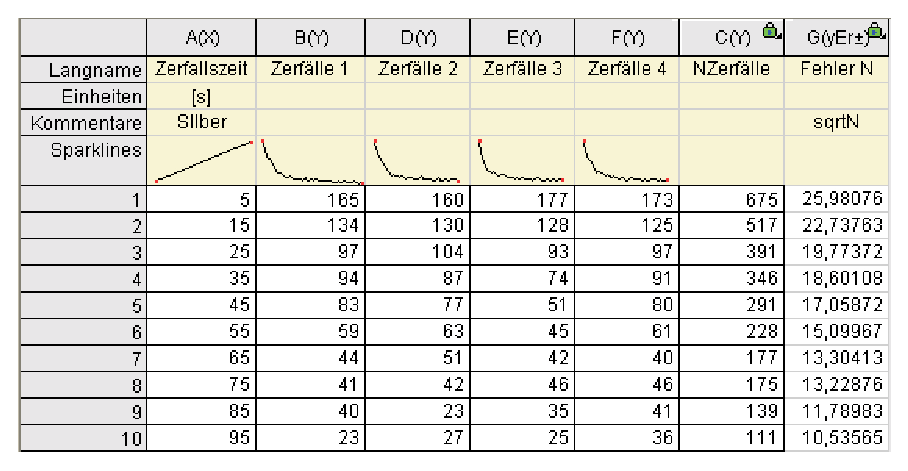
\epsfig{file=252_soft1.eps,width=11cm}
\caption{\fontsize{10}{12}\it \label{252_soft1} Ausschnitt der Arbeitsmappe.}
\end{minipage}
\end{figure}

Setzen Sie die Spalte mit dem Fehler auf Y-Fehlerbalken. Dazu die Spalte markieren, Rechtsklick und die Option \verb"Einstellungen..." aufrufen. W\"{a}hlen Sie unter \verb"Diagrammzuordnung" die Option \verb"Y-Fehler" aus. Zeichnen Sie die Zerf\"{a}lle als Funktion der Zerfallszeit mit Fehlerbalken: Spalten \verb"C" und \verb"G" markieren und unter \verb"Zeichnen" $\rightarrow$ \verb"Symbol" $\rightarrow$ \verb"Punktdiagramm" w\"{a}hlen. Durch einen Doppelklick auf die y-Achse k\"{o}nnen Sie eine logarithmische Darstellung \verb"Log10" w\"{a}hlen und geeignete x- und y- Intervalle einstellen. Beschriften Sie das Diagramm (z.B. \textit{Zerfall von Silber mit Untergrund}), drucken Sie es aus und heften Sie es in Ihr Protokollbuch.

Im n\"{a}chsten Schritt soll die Zerfallsfunktion an die Daten gefittet werden.
Klicken Sie im Menu auf \verb"Analyse" $\rightarrow$ \verb"Anpassen" $\rightarrow$ \verb"Nichtlinearer Fit" $\rightarrow$ \verb"Dialog oeffnen".
Im Dialogfenster unter \verb"Einstellungen" $\rightarrow$ \verb"Funktionsauswahl" k\"{o}nnen Sie die Fitfunktion ausw\"{a}hlen. W\"{a}hlen Sie hierf\"{u}r die bereits vorhandene Funktion \verb"ExpDec2". Sie k\"{o}nnen sich die Funktion unter dem Registerblatt  \verb"Formel" anschauen (Abbildung~\ref{252_soft2}).

\begin{figure}[h]
\begin{minipage}[c]{12cm}
\centering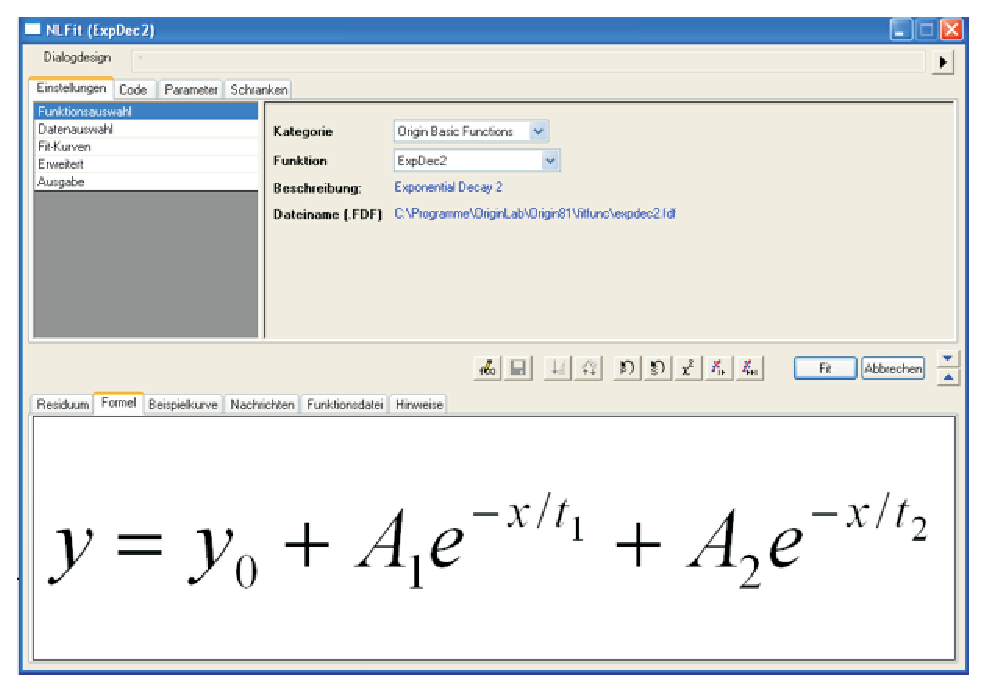
\epsfig{file=252_soft2.eps,width=11cm}
\caption{\fontsize{10}{12}\it \label{252_soft2} Funktionsauswahl im Fitdialog.}
\end{minipage}
\end{figure}

W\"{a}hlen Sie unter \verb"Datenauswahl" die zu fittenden Daten aus und ordnen Sie die Fehler zu:
\verb"Bereich 1" $\rightarrow$ \verb"y" $\rightarrow$ \verb"Gewichtung" $\rightarrow$ \verb"Zeilen".
Unter \verb"Zeilen" k\"{o}nnen Sie, falls gew\"{u}nscht, einen Datenbereich angeben, der gefittet werden soll. Ohne Angabe werden alle Daten gefittet.

Im letzten Schritt m\"{u}ssen noch sinnvolle Anfangsparameter gesetzt werden. Klicken Sie dazu auf das Registerblatt \verb"Parameter" (Abbildung~\ref{252_soft3}).
\begin{figure}[h]
\begin{minipage}[c]{12cm}
\centering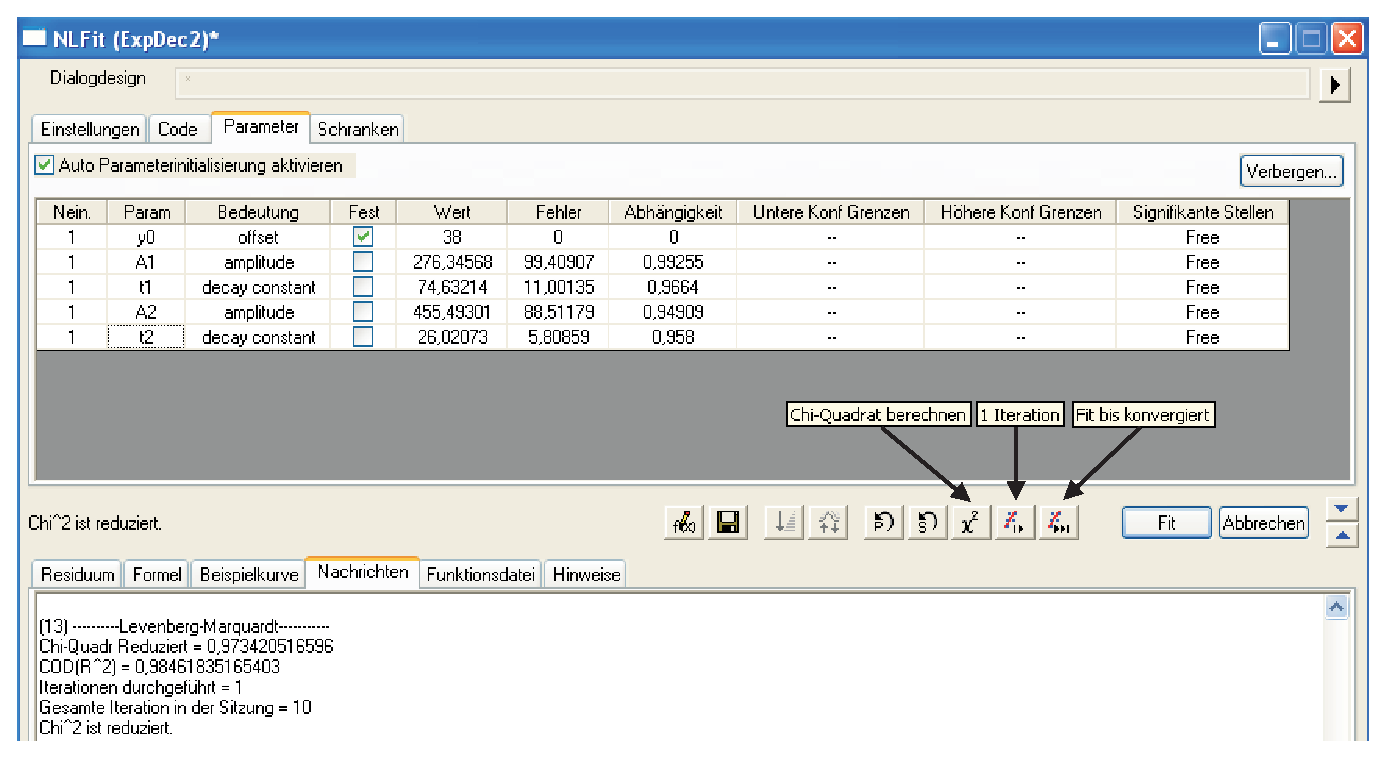
\epsfig{file=252_soft3.eps,width=\textwidth}
\caption{\fontsize{10}{12}\it \label{252_soft3} Initialisierung der Fitparameter im Fitdialog.}
\end{minipage}
\end{figure}

Origin hat bereits erste Sch\"{a}tzwerte f\"{u}r die Parameter eingef\"{u}llt, allerdings auch f\"{u}r den Parameter $y_0$, der den Untergrund bestimmt. Da wir den  Untergrund kennen, m\"{u}ssen Sie den Wert f\"{u}r $y_0$ auf die gemessene Untergrundrate setzen und den Parameter fixieren.
Klicken Sie danach auf den Knopf \begin{minipage}{5mm}

\includegraphics[height=4mm]{icon_chi2.eps}\end{minipage} und beobachten Sie wie eine Kurve in Ihr Diagramm gezeichnet wurde. Falls Sie keine Kurve sehen, m\"{u}ssen Sie die Parameter entsprechend \"{a}ndern.  Klicken Sie nun mehrfach auf den daneben liegenden Knopf \begin{minipage}{5mm}

\includegraphics[height=4mm]{icon_1it.eps}\end{minipage} f\"{u}r eine Iteration und beobachten Sie gleichzeitig die Fitkurve im Diagramm und den Wert von $\chi^2$ im Nachrichtenfenster. Falls der Fit nicht konvergiert, m\"{u}ssen Sie bessere Parameter w\"{a}hlen. Falls sich die Fitkurve den Daten ann\"{a}hert, k\"{o}nnen auf den Knopf \verb"Fit" klicken. Wenn Sie den Wechsel zum Ergebnisblatt akzeptieren, \"{o}ffnet sich eine Tabelle mit detaillierten Fitergebnissen. In das Diagramm wird die Fitkurve und eine Tabelle mit den wichtigsten Fitergebnissen eingeblendet.

Der Fehler des Untergrunds wurde in dieser Fitroutine nicht ber\"{u}cksichtigt. Dies sollen Sie nun im letzten Schritt durchf\"{u}hren.
Wiederholen Sie dazu den Fit zweimal:

\begin{enumerate}
  \item Subtrahieren Sie vom gemessenen Untergrund den 1-$\sigma$ Fehler des Untergrunds. W\"{a}hlen Sie diesen Wert als Fitparameter $y_0$ und fixieren Sie den Wert.
  \item Wiederholen Sie dies, indem Sie nun zum gemessenen Untergrund den 1-$\sigma$ Fehler des Untergrunds hinzu addieren.
\end{enumerate}

Sie erhalten so zus\"{a}tzlich zwei unterschiedliche Werte $t^-, t^+$ f\"{u}r die jeweiligen Zerfallszeiten. Berechnen Sie aus diesen Werten die Differenzen $|t-t^-|$ und $|t-t^+|$ wobei $t$ die urspr\"{u}nglich bestimmte Zerfallszeit darstellt. Der Fehler der jeweiligen Zerfallszeit erhalten Sie nun, indem Sie den  Mittelwert der berechneten Differenzen quadratisch zum Fehler aus dem ersten Fit addieren.
Drucken Sie am Ende das Diagramm aus und geben Sie die Lebensdauern und Halbwertszeiten der beiden Silberatome mit Fehler an. Vergleichen Sie diese mit den Literaturwerten (aus der Nuklidkarte). Diskutieren Sie die Fitwahrscheinlichkeit aus dem Wert von $\chi^2$. Die Wahrscheinlichkeiten finden Sie im Anhang des Statistikversuchs.



\item Indiumzerfall:\\
\\
Die Auswertung der Indiummessung erfolgt analog zu der Silbermessung. Den Untergrund m\"{u}ssen Sie f\"{u}r ein zwei Minuten Intervall bestimmen. Als Fitfunktion  k\"{o}nnen Sie
die bereits vorhandene Funktion \verb"ExpDec1" ausw\"{a}hlen.

Hinweis: Sie werden im Diagramm vermutlich festgestellt haben, dass der Messwert im ersten Bin (bei 1 Minute) deutlich \"{u}ber der Fitkurve liegt, auch wenn das nicht unbedingt signifikant sein muss.  Schauen Sie bei ihren Kollegen nach. Falls dies dort auch der Fall ist,  sollten Sie sich \"{u}berlegen ob es eine systematische Ursache daf\"{u}r gibt. Schauen sie sich die Zerfallsdaten von $^{116}$In in in der Nuklidkarte nochmals an. Falls Sie einen Grund finden, dann sollten sie den ersten Messwert bei der Anpassung nicht benutzen.

\end{enumerate}
\newpage
\section{Anhang}
\begin{figure}[h]
\begin{minipage}[c]{12cm}
\centering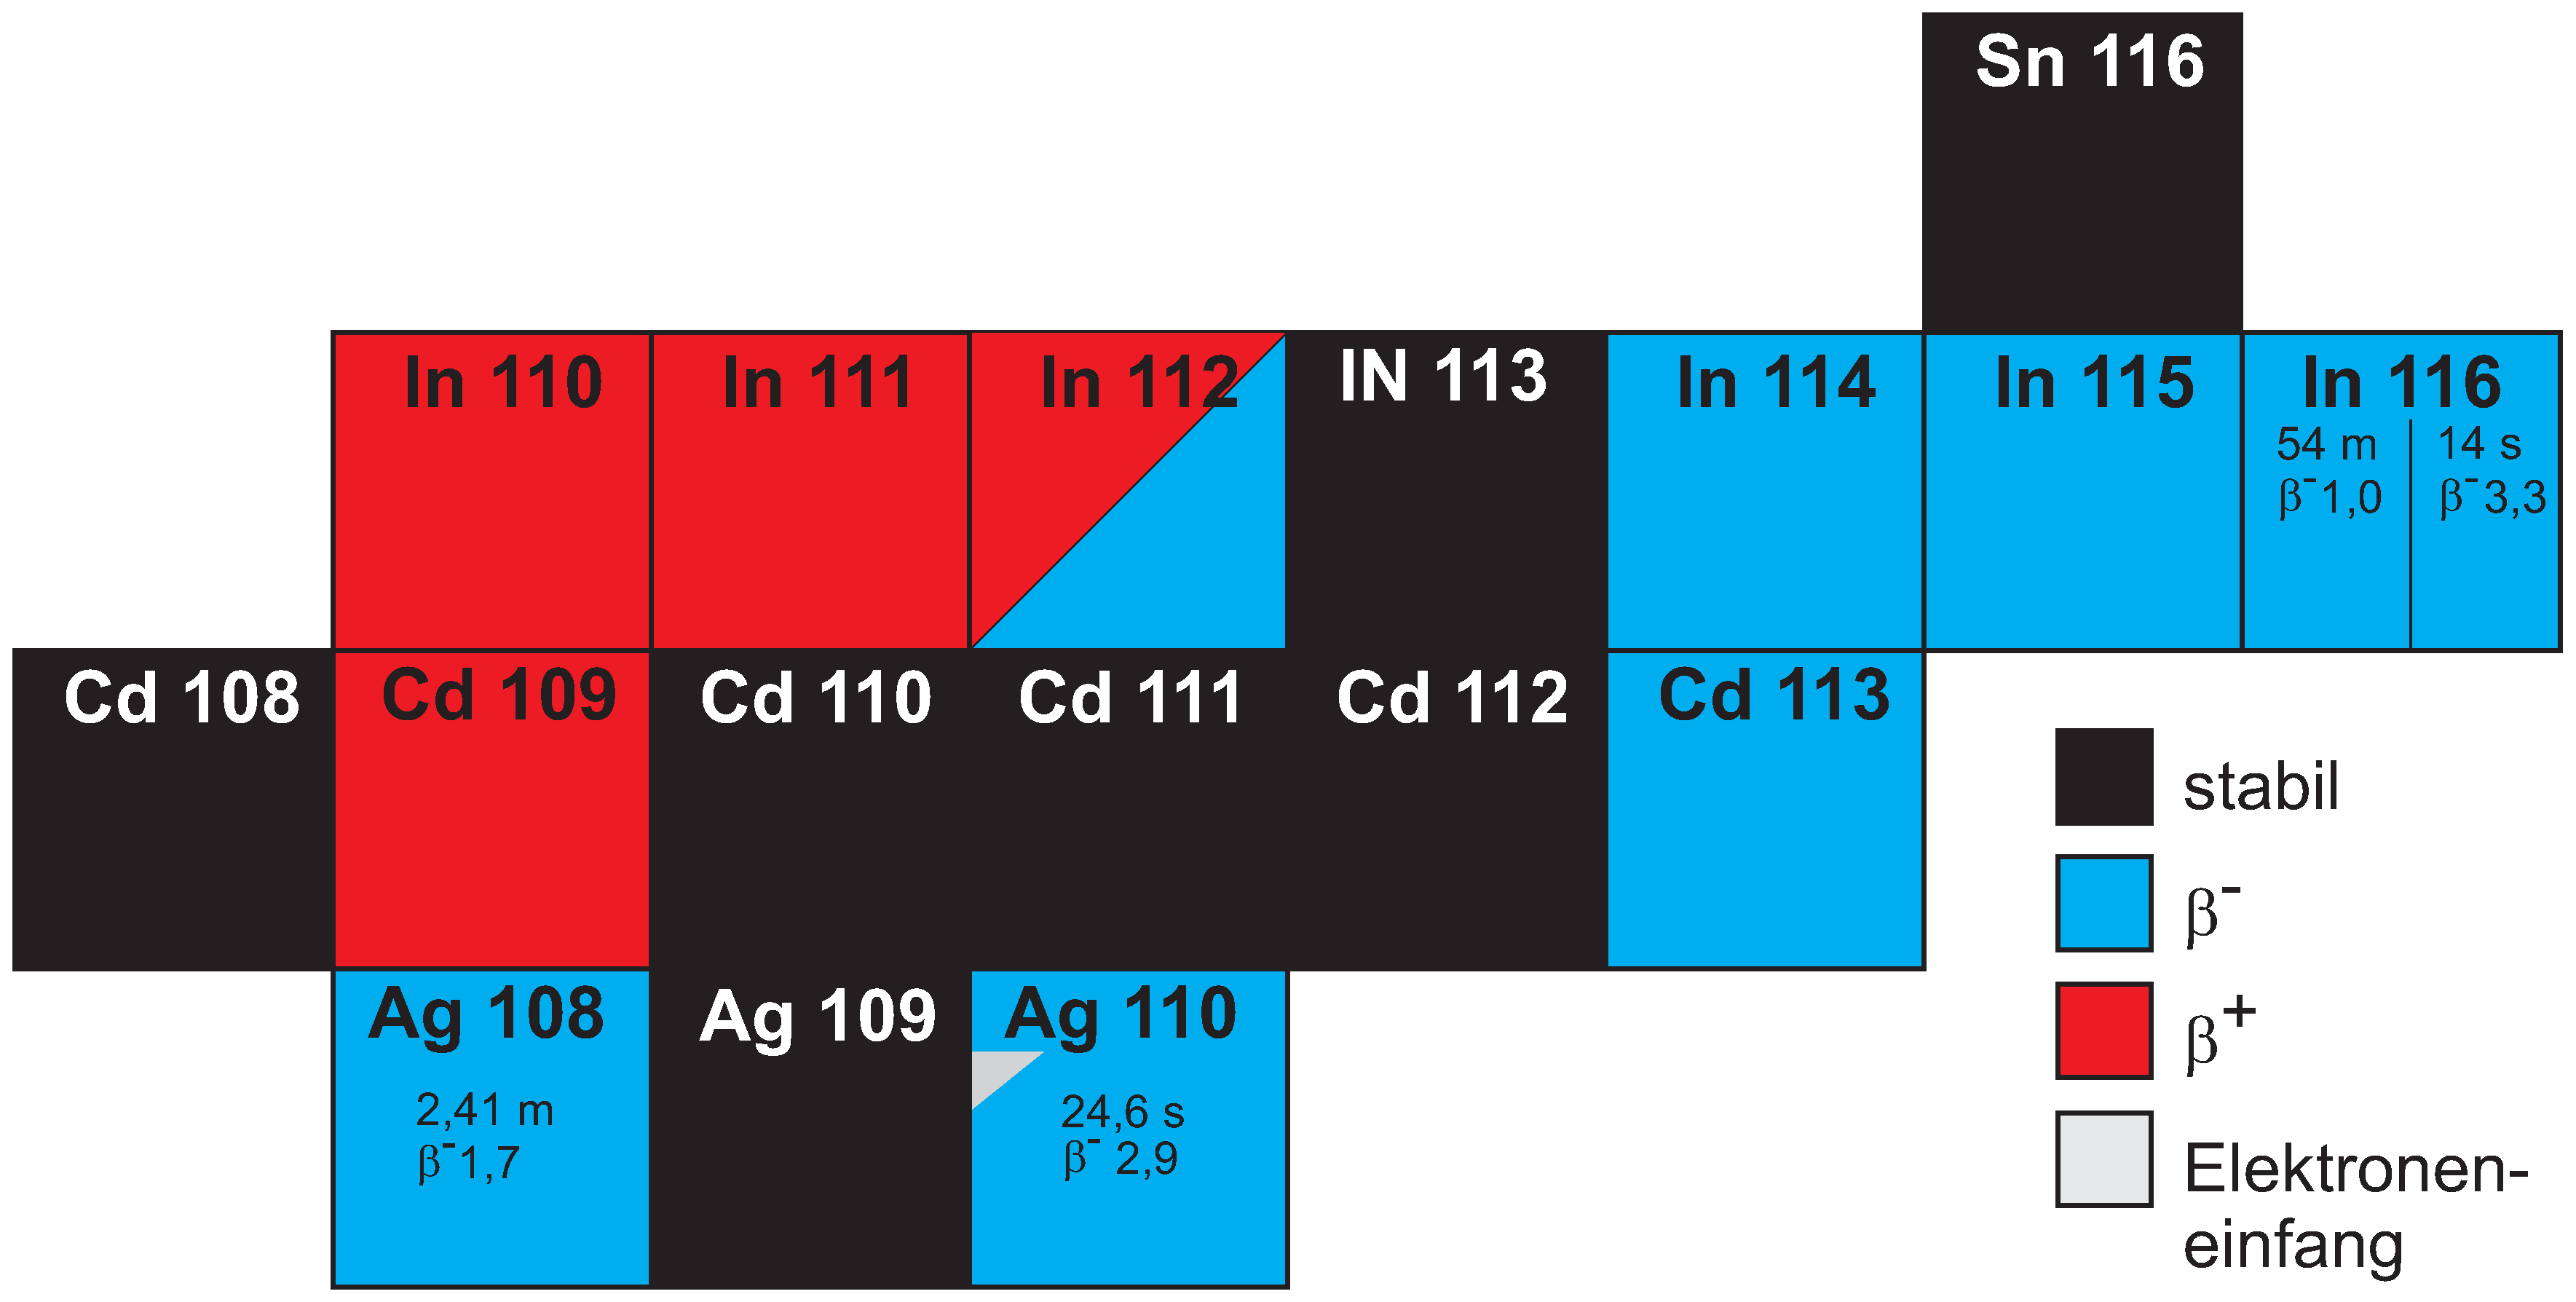
\epsfig{file=252_nuklidkarte.eps,width=\textwidth}
\caption{\label{252_nuklidkarte}\fontsize{10}{12}\it Ausschnitt Nuklidkarte. Die Farben symbolisieren die verschiedenen Zerfallsarten. Bei den hier interessierende Isotopen ist zus\"{a}tzlich noch die Halbwertszeit, sowie die Energie der emittierten Strahlung angegeben (in MeV).}
\end{minipage}
\end{figure}


 \setcounter{section}{0}

\setcounter{figure}{0}

\setcounter{equation}{0}

\setcounter{footnote}{0}

 \setcounter{section}{0}
\end{document}


https://lp.uni-goettingen.de/get/text/4433
http://www.ipkm.tu-bs.de/dokumente/Versuch_10.pdf
